% !Mode:: "TeX:UTF-8"
\section{研究背景及意义}
\subsection{课题研究背景}
\subsubsection{软件定义网络SDN}
%在传统的网络架构中,数据平面和控制平面没有分离,是集成在同一处的硬 件系统上的。这使得新业务在引进时十分不便,一方面需要在路由交换、数据处 理等业务之外进行相关处理工作,另一方面还需要在网络技术、支撑软件与业务 创建软件等软件相关方面进行相应地设计与研究。这样一来,使得网络运营商需 要增加成本来进行运营维护,也阻碍了客户要求的对业务作出迅速响应的请求, 同时也妨碍了业务本身的创新。
众所周知,相比发展迅速的计算机产业,网络产业的创新十分缓慢。每一个创新都 需要等待数年才能完成技术标准化。为了解决这个问题,SDN创始人Nick McKeown教 授对计算机产业的创新模式和网络产业的创新模式进行了研究和对比。在分析了计算机 产业的创新模式之后,他总结出支撑计算机产业快速创新的如下三个因素。

(1)	计算机工业找到了一个面向计算的通用硬件底层:通用处理器,使得计算机 的功能可以通过软件定义的方式来实现。

(2)	计算机功能的软件定义方式带来了更加灵活的编程能力,使得软件应用的种 类得到爆炸式的增长。

(3)	计算机软件的开源模式,催生了大量的开源软件,加速了软件开发的进程,推动了整个计算机产业的快速发展,Linux开源操作系统就是最好的证明。

相比之下,传统的网络设备与上世纪60年代的IBM大型机类似,网络设备硬件、 操作系统和网络应用三部分紧耦合在一起组成一个封闭的系统。这三部分相互依赖,通 常隶属于同一家网络设备厂商,每一部分的创新和演进都要求其余部分做出同样的升级。 这样的架构严重阻碍了网络创新进程的开展。如果网络产业能像当今计算机产业一样, 也具备通用硬件底层、软件定义功能和开源模式三要素,一定能获得更快的创新速度, 最终像计算机产业一样取得空前的发展。

正是在这种思路的影响下,McKeown教授团队提出了个新的网络体系结构:SDN在SDN架构中,网络的控制平面与数据平面相分离,数据平面将变得更加通用化,变 得与计算机通用硬件底层类似,不再需要具体实现各种网络协议的控制逻辑,而只需要 接收控制平面的操作指令并执行即可。网络设备的控制逻辑转而由软件实现的SDN控 制器和SDN应用来定义,从而实现网络功能的软件定义化。随着开源SDN控制器和开 源SDN开放接口的出现,网络体系结构也拥有了通用底层硬件、支持软件定义和开源 模式:个要素。从传统网络体系结构到SDN网络体系结构的演进关系如图\ref{fig:SchematicDiagram4EvolutionFromTraditionalNetworkArchitecture2SDNArchitecture}所示。
\begin{figure}[htbp]
\centering
% Requires \usepackage{graphicx}
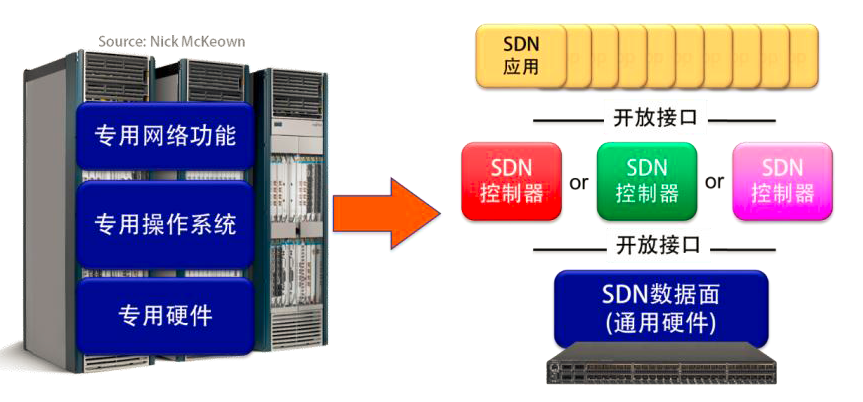
\includegraphics[width=3.0in]{figures/SchematicDiagram4EvolutionFromTraditionalNetworkArchitecture2SDNArchitecture}
  \caption{传统网络架构向SDN架构演进示意图}
  \label{fig:SchematicDiagram4EvolutionFromTraditionalNetworkArchitecture2SDNArchitecture}
\end{figure}



有人认为,SDN就是数控分离;有人认为,SDN就是OpenFlow;还有人认为只要 支持软件编程控制的网络就是SDN。不同的人对SDN有着不一样的理解,正如一千个 人眼中有一千个哈姆雷特。为探究SDN的准确定义,我们将以ONRCW (OpenFlow NetworkResearch Center,开放网络研究中心)和 ONF[2] (OpenNetworkingFoundation, 开放网络基金会)对SDN的定义为切入点,深入探讨SDN的本质,一层一层揭开SDN 的神秘面纱,直到看清SDN的庐山真面目。ONRC是SDN创始人斯坦福大学教授Nick McKe〇wn[3]和加州大学伯克利分校教授 Scott Shenker,以及大名鼎鼎的Larry Peterson教授[5哄同创建的研究架构。ONRC对SDN的定义是:“SDN是一种逻辑集中控制的新网络架构,其关键属性包括:数据平面 和控制平面分离;控制平面和数据平面之间有统一的开放接口 OpenFlow。”在ONRC的 定义中,SDN的特征表现为数据平面和控制平面分离,拥有逻辑集中式的控制平面,并 通过统一而开放的南向接口来实现对网络的控制。ONRC强调了“数控分离”,逻辑集 中式控制和统一、开放的接口。

相比ONRC对SDN的定义,另一个重要的组织ONF对SDN定义做出了不同的描 述。ONF是Nick McKeown教授和Scott Shenker教授联合多家业界厂商发起的非营利性 开放组织,其工作的主要内容是推动SDN的标准化和商业化进程。ONF认为:“SDN 是一种支持动态、弹性管理的新型网络体系结构,是实现高带宽、动态网络的理想架构。 SDN将网络的控制平面和数据平面解耦分离,抽象了数据平面网络资源,并支持通过统 一的接口对网络直接进行编程控制”。相比之下,ONF强调了 SDN对网络资源的抽象能 力和可编程能力。

本质上,这两个组织给出的SDN定义并没有太大的差别,都强调了 SDN拥有数据 平面和控制平面解耦分离的特点,也都强调了 SDN支持通过软件编程对网络进行控制 的能力。但是ONRC更强调数控分离和集中控制等表现形式,而ONF则强调抽象和可 编程等功能。
从ONRC和ONF对SDN的定义中可以了解到:SDN不仅重构了网络的系统功能, 实现了数控分离,也对网络资源进行了抽象,建立了新的网络抽象模型。SDN主要有如 下三个特征。

(1)	网络开放可编程:SDN建立了新的网络抽象模型,为用户提供了一套完整的 通用API,使用户可以在控制器上编程实现对网络的配置、控制和管理,从而加快网络 业务部署的进程。

(2)	控制平面与数据平面的分离:此处的分离是指控制平面与数据平面的解耦合。 控制平面和数据平面之间不再相互依赖,两者可以独立完成体系结构的演进,类似于计 算机工业的Wintel模式,双方只需要遵循统一的开放接口进行通信即可。控制平面与数 据平面的分离是SDN架构区别于传统网络体系结构的重要标志,是网络获得更多可编程能力的架构基础。

(3)逻辑上的集中控制:主要是指对分布式网络状态的集中统一管理。在SDN架 构中,控制器会担负起收集和管理所有网络状态信息的重任。逻辑集中控制为软件编程 定义网络功能提供了架构基础,也为网络自动化管理提供了可能。

因此,只要符合以上三个特征的网络都可以称之为软件定义网络。在这三个特征中, 控制平面和数据平面分离为逻辑集中控制创造了条件,逻辑集中控制为开放可编程控制 提供了架构基础,而网络开放可编程才是SDN的核心特征。
一般来说,SDN网络体系结构主要包括SDN网络应用、北向接口、SDN控制器、 南向接口和SDN数据平面共五部分,如图\ref{fig:SDNArchitectureDiagram}所示。

\begin{figure}[htbp]
\centering
% Requires \usepackage{graphicx}
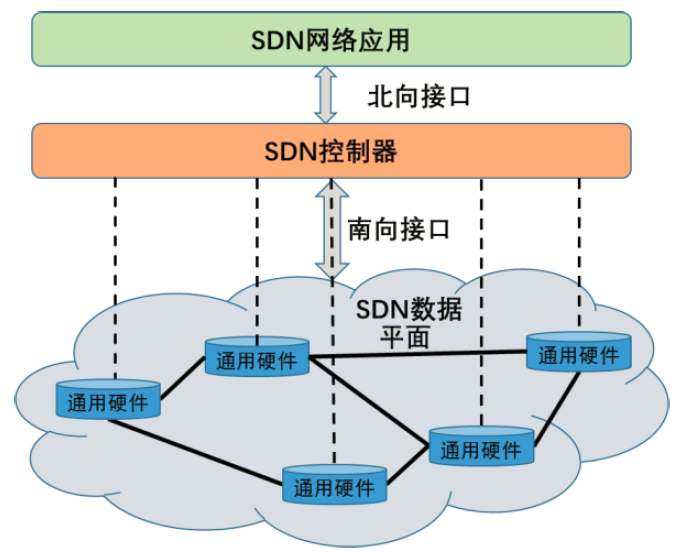
\includegraphics[width=3.0in]{figures/SDNArchitectureDiagram}
  \caption{SDN体系架构图}
  \label{fig:SDNArchitectureDiagram}
\end{figure}

现代电信网络提供多种高速通信。通过大规模的面向连接和分组交换的网络提供服务运行在光网络之上,数字用户线路(DSL),电缆连接甚至无线地面和卫星连接。因为社会很大程度上依赖于现代电信网络,已经做了很多工作来防止网络故障,例如,通过改善设备环境和材料的物理方面。然而,过去一个世纪的电信显示,网络组件仍然经常出现故障。[82]。不论采取了哪些预防性保护措施,网络节点和链接将最终失灵,并停止运作。





SDN
TE
TE 与 SDN的结合




随着通信技术的快速发展,网络链路带宽得到不断扩充。目前全球至少有来自20 多个国家的53个运营商已经部署或正在考虑部署 400 GB/s 的骨
干网络[1]。高速骨干网链路即使短暂的故障也会造成
大量的数据包丢弃,严重影响通信质量。根据对ISP
的观察,骨干网链路一年内大约有30%的概率会出
现故障[2],表明链路故障是网络中较为普遍的现象。
因此,加快故障的恢复速度,降低故障造成的业务
丢弃已成为当前研究亟待解决的问题。
网络故障主要表现为链路故障,链路故障恢复
策略可分为主动式和被动式两种[3,4]。被动式策略在
网络故障后动态自适应地进行全网资源重分配,但
路由重新收敛花费较多的时间而不可接受。因此目
前故障快速恢复研究以主动式策略为主,通过提前
对网络进行资源规划和预留,使得故障时能迅速切
换,如基于多拓扑[5]和基于备份路径的故障恢复技
术。多拓扑技术需要配置多个拓扑子层,路由存储
消耗大;基于备份路径的故障恢复技术提供端到端
路径重路由,在全局范围内进行流量分配,易于基
于现有协议实现。因此,备份路径技术是当前故障
恢复领域研究的热点[6-11]。
故障恢复的本质在于维持故障链路承载流量的
传输,因此应从流量持续传输角度解决故障恢复问
题。大部分故障恢复工作集中在如何选择可靠备份
路径上,且一般利用单一备份路径进行故障恢复。
然而当流量超出备份路径可用带宽时,单一备份路
径无法满足故障恢复的要求。受到这一启发,文献
[8]将多路径技术引入到故障恢复中,采用多条备份
路径共同承担流量,减少了流量的丢弃。在此基础
上,文献[9]提出一种结合故障恢复与流量工程的网
络结构,在多路径故障恢复基础上进行流量工程优
化,其目的是进行负载均衡,且假设备份路径可用
带宽满足故障恢复需求。文献[10]考虑了不同故障状
况,通过将重路由流量分配给有跳数限制的多条备
份路径,在网络投入运行之前就设计好应对各种故
障场景的最低容量备份网络。文献[11]提出一种跨层
故障恢复模型,考虑了备份链路的可靠性,提升了
故障恢复成功率。然而,上述故障恢复算法大都以
最大化重路由为目标,未考虑恢复后的流量是否满
足用户的需求。但是经由备份路径的重路由流量即
使最终传输成功,由于时延超时、链路过载等原因,
也无法满足业务的服务质量需求(Quality of Service,
QoS),属于无效流量。虽然文献[12]提出了一种满
足QoS 约束的自适应调整的多路径路由,但未考虑
故障恢复问题。因此,目前已提出的大部分链路故
障恢复算法不能很好地确保业务的服务质量。
为此,本文针对QoS 约束下的链路故障恢复问
题进行研究,即在网络可用带宽和业务时延需求约
束下进行最大化重路由流量问题求解。首先基于多
备份路径策略建立概率关联故障模型和重路由流量
丢弃优化目标,并构建QoS 约束的故障多备份路径
恢复问题的数学优化模型。然后,设计QoS 约束的
链路故障多备份路径恢复算法(Multiple backup
Paths Recovery for link failure with QoS constrain
algorithm, MPR-QoS) 对此问题进行求解。
MPR-QoS 算法在构建单条备份路径时,利用改进
的QoS 约束的k 最短路径法进行拼接,并以最大化
减少重路由流量丢弃为目标,且分配给高优先级链
路更多的保护资源。此外还证明了算法的正确性并
对时间空间复杂度进行了分析。最后,在NS2 仿真
环境下从故障恢复率、重路由流量QoS 满足率、链
路过载率和算法运行时间等方面验证了本文算法的
优越性。

\subsubsection{网络功能虚拟化NFV}



并且由于目前虚拟SDN 网络拓扑的部署会增加SDN运营商的配置开销,所以出现了 SDN虚拟化层的解决 方案,协调SDN虚拟网络的部署和管理。SDN管理程序可以生成并安装SDN虚拟 网络启动所需的转发表,并协调修改交换机流表以实现资源的迁移,将多个虚拟 流表配置并合并到单个交换机上以便支持任意的网络拓扑。


另一方面,由于互联网的迅猛发展,己经导致了我们生活各个方面的虚拟化, 虚拟化这一现象在我们身边司空见惯。现在大热的虚拟现实(Virtual Reality,VR) 技术也是利用计算机操作,让我们身临其境地感受一个三维的虚拟世界。在网络 研究领域中,“网络虚拟化”是•个重要的未来网络的研究方向。虽然世界上的第一 个虚拟局域网早在上世纪90年代就出现了,但是科技领域对于网络虚拟化这项技 术的探索一直持续到现在,从来没有停止过,其实它最初的功能是用作一个简单的开关,到后来慢慢应用到相互独立的软件环境和硬件环境。在N络虚拟化技术 中,一般认为网络虚拟化是使得多个逻辑网络共享一个物理网络,不过网络设计 中原有的层次结构不会被破坏,同样不被破坏保留的还有网络中的数据通道以及 所能提供的服务,所有这些特点都会让用户感觉自己在独享物理网络[31

为了获得当前和未来云计算的成功,网络虚拟化也是其中的关键,而SDN是 网络可编程性的关键,SDN由于其集中控制的特性,它最适合的领域应该是数据 中心中网络虚拟化的应用。SDN要求集中控制,网络虚拟化也同样要求集中化控 制,网络虚拟化可以为数据中心的每个“租户”提供自己的网络拓扑并控制其流量, 这种特性使得两者很自然地结合到一起了。SDN 可以在控制器应用和交换机转发 表之间提供标准接口,因此,是网络虚拟化的自然平台。然而,支持具有不同拓 扑和控制器应用的许多租户提出了可扩展的挑战性,所以SDN虚拟网络的概念应运而生,其中,虚拟网络服务是SDN虚拟网络的一部分,也是部署防火墙、均衡 负载、网络路由和虚拟专用网(Virtual private network, VPN)等按需求提供功能的 应用软件。在软件中,虚拟化网络服务消除了对昂贵的物理、专有和固定网络的 需要,这些设备都缺乏数据中心所需的灵活性和可扩展性。并且,现在的云计算 技术大大减缓了创建新网络服务的压力,同时,诸如网络创新的全球实验环境可 以让研宄人员在共享基础设施的分片上进行大规模的实验,让租户共亨物理资源, 虚拟化技术势必成为了这些基础架构中的关键。

SDN架构和网络虚拟化技术都希望当今通信网络的灵活性和可编程性能够得 到增强,结合这两种技术能够提高网络资源的有效利用率。在现在已有的基于SDN 网络虚拟化的多种解决方案中,要么是在软件中实现,要么需要特殊的硬件支持, 如现有的FLowN架构就会给用户这样一种错觉,它提供了自己的拓扑、地址空间 和控制器,并且利用数据库技术对虚拟网络和物理交换机的映射进行了有效地存储和操作,而HyperFlex可以在软件中添加控制平面隔离功能来提供控制平面的虚 拟化,它是一种SDN管理架构,它提供的隔离功能可以确保在每个SDN虚拟网络 之间共亨控制平面的资源,同时还可以避免管理资源耗尽的现象141。
在SDN网络虚拟化中,一项很重要的技术是虚拟网络的映射,在将虚拟网络 映射到底层的物理设备时,对于不同的虚拟网络和物理网拓扑,设计不同的映射 算法,会得到不同效率的映射方案,如何映射以确保网络资源的高效利用以及网 络的负载均衡,也是现在和未来网络研究的方向,同时也是本文要攻克的一个难 题。通过与国内某大型公司合作,本课题结合了实际项0,在研究SDN网络虚拟 化技术以及基于最短分离路径和有必经约束路由算法研究的基础上,进一步研宄






SDN作为新型网络架构,数据网络中心作为未来网络研究的重要领域,SDN在数据中心网络的应用具有研究意义。

本文结合实际情况,以基于SDN网络的多路径路由技术作为课题的研究方向,主要研究以三个方面内容。


\subsection{课题研究目的和意义}
服务器和存储器的虚拟化带来了网络规模的增大和流畅性的提高,从而进一 步加大了自动化、多租户和多路径的迫切性,也带来了网络虚拟化的需求。虚拟 化的总体思想就是要创建一个运行在被抽象的实际物理实体之上的更高层次的抽 象m。有了网络虚拟化,网络管理员不仅可以随时随地选择创建N络,还能够任意 扩展和收缩已经存在的网络。智能的虚拟化软件在完成这些任务时,位于上层的 虚拟网络不需要知道底层物理拓扑发生了什么变化,上层虚拟网络在向底层虚拟 网络映射时,为了达到低成本高收益的效果,需要找到最有效的映射算法。而由 于SDN的集中控制性能,相比传统的分布式算法,集中控制器可以更好地执行最 优路径的计算,这是因为:(1)它有一个更稳定的网络全局视图;(2)它可以考虑更 多的因素,包括当前带宽的负载情况等;(3)它可以在服务器性能较高的内存和处 理器上执行计算,而不是在网络设备能力有限的可用内存和处理器上执行。

为了支持具有不同拓扑结构的虚拟网络,需要一种映射方法将虚拟网络映射 到物理设施,并将物理网故障如链路或交换机故障映射到虚拟网络组件,任何虚 拟化解决方案都必须快速执行这些映射操作,以便每个租户可以对其虚拟网络提 供实时控制151。在将虚拟网络映射到物理网络时,映射算法是其中的关键,在将虚 拟网络的节点和链路进行映射时,需要找到最佳路由完成资源的配置,现有的路 由算法己经很多,对于不同的应用场景,很难评判算法性能的好坏,较好的解决 办法是针对不同的应用场景设计满足要求的算法,使算法的性能和效率能够优化。 另外,在虚拟网络的映射过程中,为了使资源充分利用并且避免网络拥塞的情况, 可以从用户层面和网络层面进行负载均衡的研宂。


